\lecture{8}{20 marzo 2024}
\section{Riflessione e trasmissione}
Oggi studiamo i mezzi non omogenei per la trasmissione di onde. In questi mezzi può avvenire il fenomeno della riflessione, al contrario dei mezzi omogenei in cui l'onda si propaga senza cambiare forma. In generale, nel passaggio di un'onda fra due mezzi diversi si possono avere un'onda riflessa e un'onda trasmessa:

\begin{figure}[H]
	\centering
	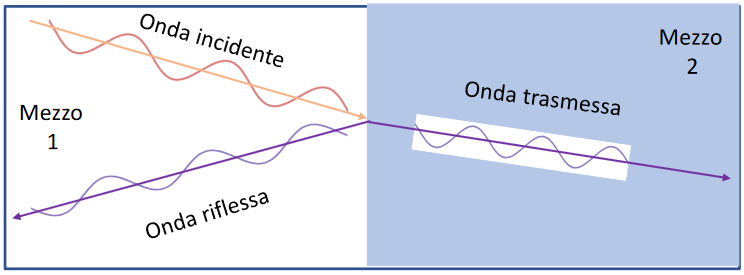
\includegraphics[width=0.6\textwidth]{screenshots/2024-03-20-09-25-33.png}
\end{figure}

Consideriamo ora una corda elastica con due densità diverse (la discontinuità è in \(x=0\)):

\begin{figure}[H]
	\centering
	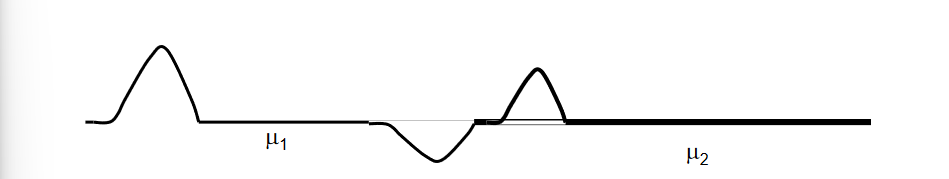
\includegraphics[width=0.8\textwidth]{screenshots/2024-03-20-09-26-28.png}
\end{figure}
Se un'onda viene diretta verso la giunzione fra i due pezzi a densità diversa si produrranno due onde: una riflessa (rovesciata nella figura) e una trasmessa (sulla destra nella figura). Per semplicità studiamo onde armoniche:

\begin{itemize}
	\item Onda incidente: \(\xi _i = A_i \cos (k_1 x -\omega t)\) 	
	\item Onda trasmessa: \(\xi _t = A_t \cos (k_2 x - \omega _2 t)\) 
	\item Onda riflessa: \(\xi _r = A_r \cos (k_1^{\prime} x + \omega _1 t)\) 
\end{itemize}

Si noti che la tensione resta la stessa in tutta la corda, pur avendo due densità di massa diverse. Le quantità che caratterizzano la corda variano fra le due parti:
\begin{align}
	\mu _1 &\neq \mu _2 \implies v_1 = \sqrt{\frac{T}{\mu _1}} \neq v_2 = \sqrt{\frac{T}{\mu _2}} & Z_1&=\sqrt{\mu _1 T}\neq Z_2 = \sqrt{\mu _2 T}   
\end{align}
Definiamo una funzione a tratti che descriva la nostra onda (ricordando che per \(x <0\) l'onda incidente e l'onda riflessa si sommano!):
\begin{figure}[H]
	\centering
	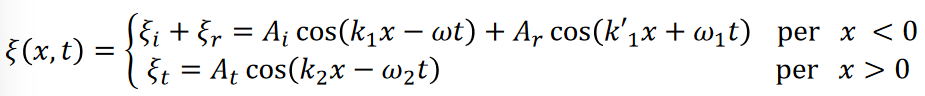
\includegraphics[width=0.8\textwidth]{screenshots/2024-03-20-09-34-41.png}
\end{figure}
Imponiamo alcune condizioni perché \(\xi (x,t)\) sia soluzione dell'equazione di D'Alembert:
\begin{enumerate}
	\item La corda è diversa per \(x>0\), tuttavia non può essere rotta: \(\xi_i(0,t) + \xi _r (0,t) = \xi _t (0,t)\)
	\item \(\xi (x,t)\) deve essere derivabile due volte per \(x=0\) e la tensione nel punto di discontinuità (quindi la forma della corda) deve essere continua nel punto di discontinuità: \(\frac{\partial \xi _i (0,t)}{\partial x} + \frac{\partial \xi _r ( 0,t)}{\partial x} = \frac{\partial \xi _t (0,t)}{\partial x}  \)    
\end{enumerate}
Applicando le condizioni 1 e 2 ottengo che:
\begin{figure}[H]
	\centering
	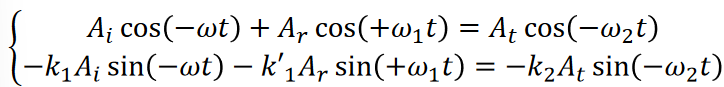
\includegraphics[width=0.8\textwidth]{screenshots/2024-03-20-09-39-42.png}
\end{figure}
Guardiamo la prima equazione: stiamo eguagliando funzioni periodiche scritte come somma di coseni, quindi per l'unicità della serie di Fourier devo concludere che \(\cos (-\omega t) = \cos (\omega _1 t) = \cos (-\omega _2 t) \implies \omega _2 = \omega _1 = \omega \rightsquigarrow k_1^{\prime} =k_1 = \omega /v_1\). Devono avere la stessa periodicità! Avevamo già detto che la periodicità temporale dell'onda non dipende dalla corda ma solo dalla sorgente.
\begin{figure}[H]
	\centering
	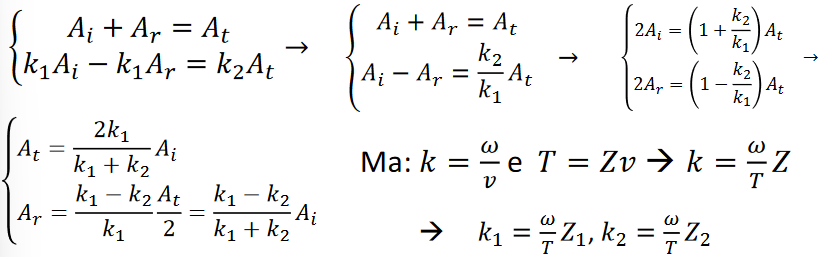
\includegraphics[width=0.8\textwidth]{screenshots/2024-03-20-09-46-35.png}
\end{figure}
Quanto trovato non è ancora sufficiente, perché sembra che a seconda delle caratteristiche dell'onda (i numeri d'onda) la riflessione e la trasmissione avvengano in maniera diversa.
\begin{formula}
	[Riflessione e trasmissione]
	Sostituendo le impedenze troviamo che le ampiezze riflesse e trasmesse non dipendono dall'onda! Si presenta solo l'impedenza, quindi valgono per tutte le onde e non solo quelle armoniche.
	\[
		\begin{dcases}
			A_t = \frac{2Z_1}{Z_1 + Z_2}A_i\\
			A_r = \frac{Z_1 - Z_2}{Z_1 + Z_2}A_i\\
		\end{dcases}
	\]
\end{formula}
Studiamo i casi limite di queste formule:
\begin{enumerate}
	\item Se \(Z_1 = Z_2\), ovvero se la corda è omogenea, non avviene riflessione: \(A_t = A_i,\ A_r = 0\) 
	\item Se \(Z_1 \gg Z_2\), \(A_t = 2A_i,\ A_r=A_i\): la corda 2 è sottile e l'onda trasmessa ha ampiezza doppia di quella incidente, mentre l'onda riflessa ha lo stesso segno di quella incidente.  
	\begin{figure}[H]
		\centering
		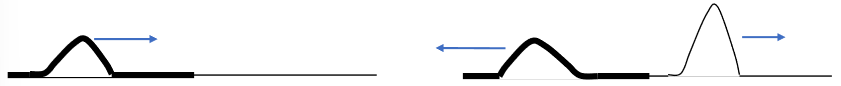
\includegraphics[width=0.8\textwidth]{screenshots/2024-03-20-09-56-02.png}
	\end{figure}
	\item Se \(Z_1 \ll Z_2\), \(A_t \to 0,\ A_r = -A_i\): la corda 2 è molto spessa e l'onda non si trasmette nella regione 2, mentre l'onda riflessa è invertita.
	\begin{figure}[H]
		\centering
		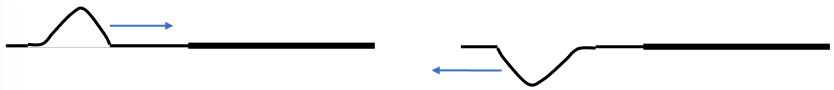
\includegraphics[width=0.8\textwidth]{screenshots/2024-03-20-09-57-19.png}
	\end{figure}  
\end{enumerate}
\subsection{Analisi energetica}
Usiamo quanto trovato ieri per trovare l'intensità delle tre onde:
\begin{figure}[H]
	\centering
	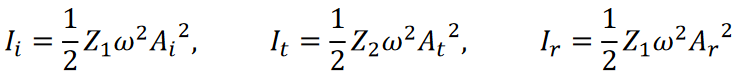
\includegraphics[width=0.8\textwidth]{screenshots/2024-03-20-09-58-18.png}
\end{figure}
Da cui si ricava che la somma delle intensità dell'onda trasmessa e dell'onda riflessa è uguale all'intensità dell'onda incidente, è un modo di scrivere la conservazione dell'energia!
\begin{figure}[H]
	\centering
	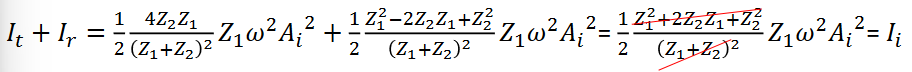
\includegraphics[width=0.8\textwidth]{screenshots/2024-03-20-10-00-41.png}
\end{figure}
\paragraph{Coefficienti R e T}
Da quanto appena ricavato è immediato definire i coefficienti che indicano quanto un'onda venga trasmessa e quanto venga riflessa.
\begin{definition}
	[Coefficienti di trasmissione e riflessione]
	Si definisce il coefficiente di trasmissione:
	\[
		T= \frac{I_t}{I_i} = \frac{4Z_2 Z_1}{(Z_1 +Z_2)^{2} }
	\]
	e il coefficiente di riflessione:
	\[
		R= \frac{I_r}{I_i}=\left( \frac{Z_1 - Z_2}{Z_1 + Z_2} \right) ^{2} 
	\]
	Dalla definizione segue immediatamente che \(T+R=1\).
\end{definition}
Vedi link Desmos per una bella simulazione: \href{https://www.desmos.com/calculator/42zmaoac6h?lang=it}{onde riflesse e incidenti}.

\paragraph{Massima onda trasmessa}
Si vede immediatamente che la massima onda trasmessa si ha per \(I_r=0 \implies A_r = 0 \implies Z_1 = Z_2\). La condizione \(Z_1\thickapprox Z_2\) è nota in fisica con il termine di \emph{raccordo delle impedenze}. In generale è più semplice ottenere questo risultato con variazioni lente (non brusche come appena studiato) dei parametri della corda:
\begin{figure}[H]
	\centering
	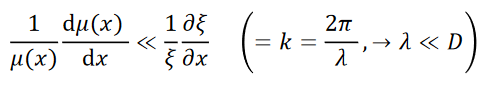
\includegraphics[width=0.4\textwidth]{screenshots/2024-03-20-10-13-59.png}
\end{figure}

\section{Onde stazionarie}
Studiamo una corda fissata a un estremo, che può essere pensato come una corda con \(\mu _0 \to \infty \). Consideriamo un'onda regressiva proveniente dalla regione \(x>0\):
\begin{figure}[H]
	\centering
	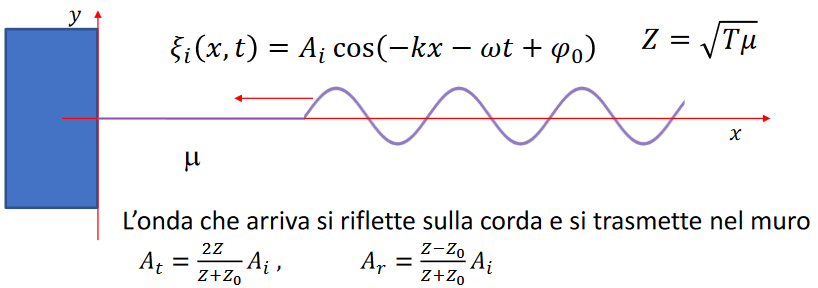
\includegraphics[width=0.8\textwidth]{screenshots/2024-03-20-10-31-36.png}
\end{figure}
Nel caso limite in cui \(Z_0 \gg Z\) abbiamo che \(A_t \to 0,\ A_r=-A_i\). L'onda riflessa è un'onda progressiva ribaltata rispetto all'onda incidente:
\[
	\xi _r(x,t)=-A_i \cos (kx -\omega t + \varphi _1)
\]
L'onda incidente e quella riflessa hanno la stessa intensità, quindi complessivamente l'onda risultante (\(\xi (x,t) = \xi _i (x,t)+\xi _r(x,t)\)) non trasporta energia. È detta \emph{onda stazionaria}. Il punto \(x=0\) è un vincolo per la corda, quindi
\begin{gather*}
	A_i [\cos (-\omega t + \varphi _0) - \cos (-\omega t + \varphi _1)]=0 \iff \varphi _1 = \varphi _0\\
	\xi (x,t) = A_i [\cos (-kx -\omega t + \varphi _0) - \cos (kx- \omega t + \varphi _0)]
\end{gather*}
Ricordando che \(\cos \alpha - \cos \beta  = -2 \sin \left( \frac{\alpha +\beta }{2} \right)\sin \left(\frac{\alpha - \beta }{2}\right)  \), possiamo scrivere in un altro modo \(\xi (x,t)\):
\begin{figure}[H]
	\centering
	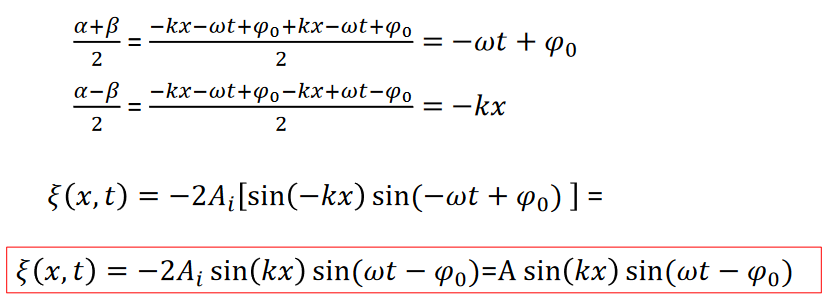
\includegraphics[width=0.8\textwidth]{screenshots/2024-03-20-10-40-21.png}
\end{figure}
La formula appena ricavata può essere ricavata come segue: ogni punto della corda oscilla nel tempo con un'ampiezza massima data da \(A \sin (kx)\). Esistono dei punti fissi (nodi) e dei punti dove l'oscillazione è massima (ventri):
\begin{itemize}
	\item Nodo: \(\sin (kx) = 0 \implies kx = n\pi \rightsquigarrow x= \frac{n \pi }{k}\) con \(n\) intero
	\item Ventre: \(\sin (kx) = \pm 1 \implies kx = \left( n+ \frac{1}{2} \right) \pi \rightsquigarrow x = \left( n + \frac{1}{2} \right) \frac{\pi }{k}  \)  
\end{itemize}

\subsection{Corda vincolata a due estremi}
\begin{figure}[H]
	\centering
	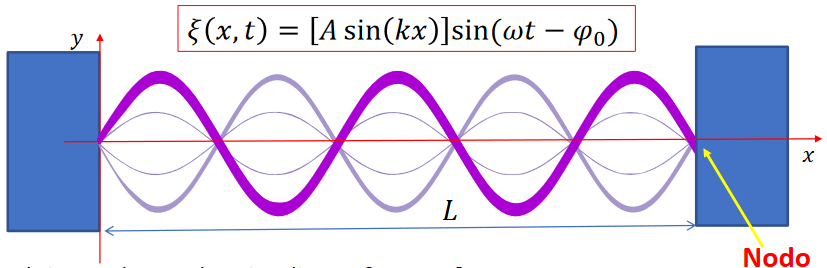
\includegraphics[width=0.8\textwidth]{screenshots/2024-03-20-10-46-00.png}
\end{figure}
La differenza con quanto fatto prima è che ora dobbiamo imporre due vincoli, in \(x=0\) e in \(x=L\), dove in ogni istante deve valere \(\xi (0,t)=\xi (L,t)=0\). Passiamo da \(k\) continui a \(k\) discreti: \(\xi (L,t) = 0 \rightsquigarrow \sin (kL)=0\rightsquigarrow k=n \pi /L\) con \(n\) intero. Stiamo \emph{quantizzando} il numero d'onda (succederà anche in meccanica quantistica!), quindi saranno quantizzate anche le lunghezze d'onda, le pulsazioni e le frequenze:
\begin{figure}[H]
	\centering
	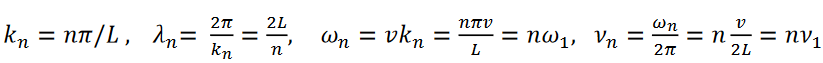
\includegraphics[width=0.8\textwidth]{screenshots/2024-03-20-10-49-52.png}
\end{figure}
\paragraph{Armonica fondamentale}
L'onda armonica ottenuta ponendo \(n=1\) è conosciuta come "armonica fondamentale".
\begin{figure}[H]
	\centering
	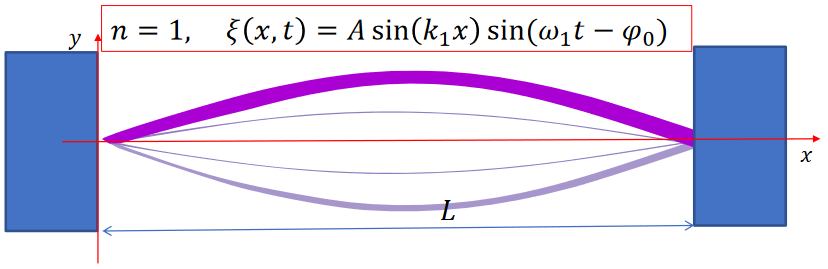
\includegraphics[width=0.8\textwidth]{screenshots/2024-03-20-10-50-49.png}
\end{figure}
\(n\) corrisponde al numero di ventri. Sommando armoniche con \(n\) diverso si possono ottenere forme diverse, se invece compare solo un'armonica parliamo di "oscillazioni di modo normale".
Le frequenze che si ottengono dalle oscillazioni di modo normale sono dette "frequenze proprie" o "autofrequenze". Qualunque onda che viaggia su una corda vincolata ai due estremi può essere espresse come combinazione lineare di armoniche fondamentali:
\begin{figure}[H]
	\centering
	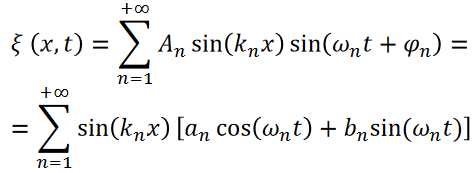
\includegraphics[width=0.4\textwidth]{screenshots/2024-03-20-10-55-47.png}
\end{figure}
\paragraph{Una chitarra}
Nella chitarra classica ci sono sei corde vincolate di diverso materiale: tipicamente tre sono di metallo e tre di nylon, avendo densità diverse permettono di coprire uno spettro più ampio di frequenze.
\[
	\nu _n = n \frac{\nu }{2L} = n \frac{1}{2L} \sqrt{\frac{T}{\mu }} 
\]
Essendo la frequenza dipendente dalla tensione, accordare la chitarra significa trovare la tensione giusta della corda per suonare la nota corretta. Suonando poggio le dita sulla tastiera per accorciare la lunghezza della corda e suonare una nota diversa.